%!TEX root = ../thesis.tex

\chapter{The Output}    
\label{App_A}
We will now share our output on our ASR Engine i.e. Kaldi. We will also share our output of Speech To Text on Vosk. Finally we will also share our output in comparison with the Google ASR library \cite{zhang_uberi_speechrecognition_nodate} for our call center test audio.

\begin{landscape}
\begin{figure}[ht]
    \centering
    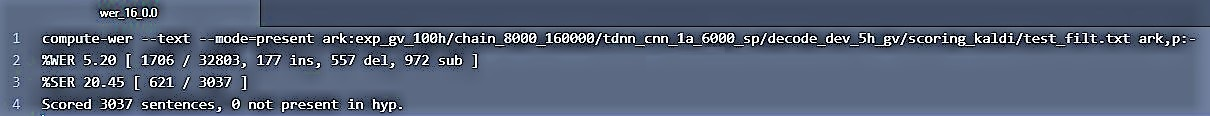
\includegraphics[width=1.45\textwidth]{img/RESULTS3.jpg}
    \caption{Output on Kaldi}
    \vspace{11pt}
    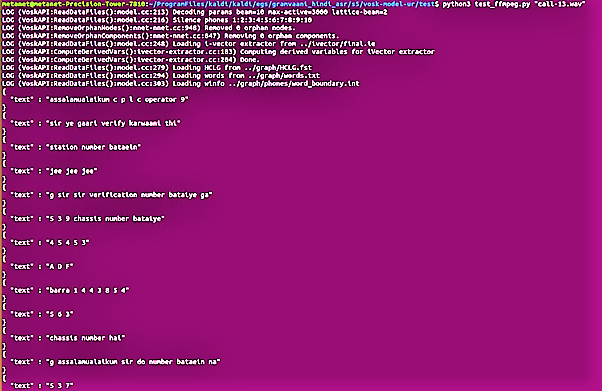
\includegraphics[width=1.2\textwidth]{img/Results-1.png}
    \caption{Output on Vosk}
    \label{fig:Result_output}
\end{figure}

\begin{figure}[ht]
    \centering
    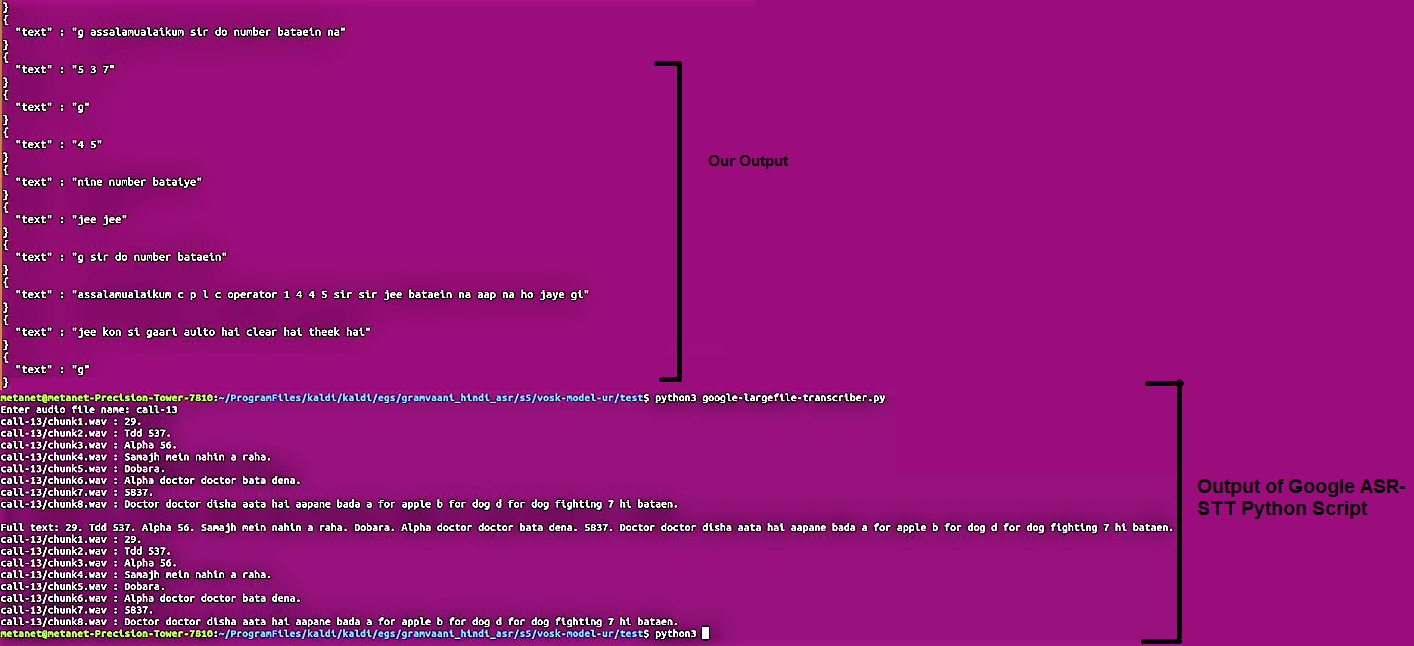
\includegraphics[width=1.5\textwidth]{img/Results-2.png}
    \caption{Our Result on our test audio data files compared to google ASR \cite{zhang_uberi_speechrecognition_nodate}. Google has Hindi Library in its Python ASR API which is why it is not able to transcribe Code-switched Urdu Audio accurately resulting in a garbage output.}    \label{fig:Result_output_compare}
\end{figure}   
\end{landscape}

\chapter{Sample Audio Pre-Processing Codes}
\label{App_B}

We used SoX and ffmpeg on our Linux System (\ref{sec:Implementation}). Instead of running a command on each, we automated the process by making a bash script which inputs  and output target directory as well as the required extensions and recursively runs the sox or ffmpeg command in all wav or mp3 files found in the directory:
\lstset{style=mycoding}
\begin{lstlisting}[language=bash, caption= Audio Pre-Processing (SoX)]
!# bin/bash
target= echo "Enter target directory: "
read target

extin= echo "enter extension of input audio file: "
read extin

extout= echo "enter extension of output audio file: "
read extout

outch= echo "enter output channel: "
read outch

dest= echo "Enter Destination file name with extension: " #Also can be used for customizing output file name along with extension
read dest

for f in "$target"/*."$extin";
do
    sox --channels "$outch" "$f"."$extin" "$f"-converted."$extout"    
done | awk 'END { printf("File count: %d", NR); } NF=NF' 
\end{lstlisting}


Same could be done with ffmpeg as well if we replace the sox line with:
\lstset{style=mycoding}
\begin{lstlisting}[language=bash, caption= Audio Pre-Processing (ffmpeg)]
ffmpeg -i "$f".wav -ss $start -to $end -c copy "$f"-converted.wav ##time format is 00:00:01 
\end{lstlisting}
 